\documentclass[conference]{IEEEtran}
\usepackage{cite}
\usepackage{amsmath,amssymb,amsfonts}
\usepackage{algorithmic}
\usepackage{graphicx}
\usepackage{textcomp}
\usepackage{xcolor}
\usepackage{booktabs}
\usepackage{multirow}
\usepackage{url}

\begin{document}

\title{Collaborative Defense in Industrial Data Spaces: A Quantum-Resistant Federated Learning Approach for Zero-Trust Edge Gateways}

\author{\IEEEauthorblockN{Alessandro De Martini}
\IEEEauthorblockA{\textit{Department of Information Systems and Technology} \\
\textit{Mid Sweden University (MIUN)}\\
Sundsvall, Sweden \\
alessandro.demartini@miun.se}
}

\maketitle

\begin{abstract}
The proliferation of the Industrial Internet of Things has dissolved traditional network perimeters, and Zero-Trust Architectures (ZTA) respond by demanding continuous verification of every request. At the industrial edge, however, Web Application Firewalls still rely on static signature sets that cannot generalise to unseen payloads, while the obvious remedy---shipping raw HTTP logs to a central model---violates the data sovereignty requirements of Industrial Data Spaces. We present a Federated Learning (FL) architecture for adaptive Zero-Trust edge gateways in which each gateway trains a lightweight linear classifier over hashed character $n$-grams of its own traffic and exchanges only model parameters with a cloud aggregator. Evaluating on 43{,}007 web paths, 8{,}013 API endpoints and 783 attack payloads drawn from SecLists, with train and test sets disjoint at the level of unique payloads, we find that the benefit of federation depends critically on how heterogeneity is distributed: when nodes differ by threat campaign alone, federated averaging lands between the isolated silos rather than above them. When nodes instead differ in their benign traffic profile---a public web gateway and an API gateway facing a shared threat landscape---the federated model outperforms every isolated silo simultaneously, reaching a ROC-AUC of 0.985 against 0.977 and 0.982, with 100\% XSS recall and 79.2\% SQLi recall at a 0.1\% false-positive budget. We further show that coordinate-wise median aggregation preserves 0.984 ROC-AUC when two of seven nodes upload sign-flipped weights, a setting in which plain federated averaging collapses to 0.263. On a Raspberry Pi~4, the resulting pure-Python inferencer sustains 452 requests per second at 0.229\,ms per classification within a 10.4\,MB resident set, and ML-KEM-512 key encapsulation costs 0.162\,ms, making post-quantum protection of the weight channel effectively free. Because each synchronisation transfers a fixed 1{,}040 bytes irrespective of inspected volume, bandwidth to the cloud falls by 99.94\% at the measured throughput.
\end{abstract}

\begin{IEEEkeywords}
Federated Learning, Zero-Trust, Edge Computing, Industrial IoT, Byzantine Robustness, Post-Quantum Cryptography, Data Sovereignty
\end{IEEEkeywords}

\section{Introduction}
The transition towards Industry 4.0 has interconnected millions of cyber-physical systems, and with them expanded the attack surface far beyond what a hardened network perimeter can contain. Legacy security paradigms assume that actors inside the local network are trustworthy; Zero-Trust Architecture (ZTA) discards that assumption and requires every request to be verified on its own merits~\cite{zheng2019,nist800207}.

Implementing ZTA at the industrial edge is harder than stating it. The Web Application Firewalls and intrusion detection systems deployed on IoT gateways are typically signature-based~\cite{modsecurity}, requiring manual rule updates and generalising poorly to polymorphic or previously unseen payloads. Machine learning offers an alternative, but training a robust model conventionally means aggregating raw traffic in a central repository. In an Industrial Data Space such as Gaia-X~\cite{gaiaX2021}, forwarding HTTP payloads that embed proprietary API queries, authentication tokens and process telemetry is precisely what the governance model forbids.

Federated Learning (FL)~\cite{mcmahan2017} resolves the tension by decentralising training: nodes compute model updates locally and transmit only parameters. Applied to WAFs, this promises collaborative defense---a gateway in Sweden benefiting from an attack first observed in Italy, with no raw payload leaving either site.

That promise is usually asserted rather than measured, and our results show it does not hold unconditionally. We find that the *axis* along which data is non-IID determines whether federation helps at all. Partitioning nodes by threat campaign---the standard framing, in which one node sees only XSS and another only SQLi---produces a federated model that sits between the two silos rather than above them, which is the behaviour predicted for FedAvg when local optima diverge~\cite{li2020convergence}. Partitioning nodes by benign traffic profile, with a shared threat landscape, is what makes federation win outright.

The contributions of this paper are:
\begin{itemize}
    \item We design a Federated Zero-Trust gateway architecture built on hashed character $n$-gram features, cheap enough for a pure-Python inferencer on ARM hardware yet expressive enough to separate attack classes (Section~\ref{sec:arch}).
    \item We show experimentally that the non-IID axis, not merely the presence of non-IID data, decides whether federation outperforms isolated training, and we report the negative result for the attack-campaign split alongside the positive one for the traffic-domain split (Section~\ref{sec:design-space}).
    \item We replace naive averaging with coordinate-wise median aggregation and measure its Byzantine resilience directly, with $K=7$ nodes of which $f=2$ are malicious (Section~\ref{sec:byzantine}).
    \item We profile the complete system on physical Cortex-A72 hardware---inference latency, resident memory, sustained throughput, and the cost of ML-KEM-512 key encapsulation---and derive the bandwidth regime in which federation is actually cheaper than log shipping (Section~\ref{sec:hardware}--\ref{sec:bandwidth}).
\end{itemize}

Section~\ref{sec:related} reviews related work, Section~\ref{sec:model} defines the system and threat model, Section~\ref{sec:arch} presents the architecture, Section~\ref{sec:crypto} addresses gradient privacy and post-quantum transport, Section~\ref{sec:setup} describes the testbed, Section~\ref{sec:eval} reports results, and Sections~\ref{sec:discussion}--\ref{sec:future} discuss limitations and future work.

\section{Background and Related Work}
\label{sec:related}
Signature-based detectors such as Snort~\cite{snort} and Suricata~\cite{suricata} remain the industrial default, but their reliance on curated rules leaves a window on every novel payload. Learned detectors close that window at the cost of computation: deep models for edge intrusion detection~\cite{wang2020} achieve strong accuracy but carry memory and latency footprints that embedded gateways cannot absorb. We therefore restrict ourselves to a linear classifier over an explicit, cheaply computable feature map.

Federated Learning was introduced by McMahan \textit{et al.}~\cite{mcmahan2017} and has since been surveyed extensively~\cite{kairouz2021,yang2019,li2020}. Within security it has been applied to malware detection and to stealthy-attack detection in IoT networks~\cite{sun2020,nguyen2021}, and its privacy and security properties have been surveyed by Mothukuri \textit{et al.}~\cite{mothukuri2021}. Its use for dynamic WAF adaptation under Zero-Trust remains comparatively unexplored.

Two lines of work bound what FL can claim. First, convergence under non-IID data is provably slower and can be worse than local training when client objectives diverge~\cite{li2020convergence}; our attack-split result is an instance of exactly this. Second, model updates leak: gradients can be inverted to recover training inputs~\cite{zhu2019}, and the standard mitigation is differentially private training with clipped, noised updates~\cite{abadi2016}.

Byzantine robustness in FL has produced a family of aggregation rules---Krum~\cite{blanchard2017}, coordinate-wise median and trimmed mean~\cite{yin2018}---all of which share the requirement that honest clients outnumber malicious ones by a stated margin. Fang \textit{et al.}~\cite{fang2020} show that such rules can still be defeated by optimised attacks; our evaluation uses a straightforward sign-flip adversary and does not claim resistance to the optimised variants. For communication cost, gradient quantisation~\cite{alistarh2017} is the standard lever, which we quantify here in terms of $n$-gram dimensionality instead.

Hashing features into a fixed-width vector is the hashing trick of Weinberger \textit{et al.}~\cite{weinberger2009}; it gives us a constant-size model independent of vocabulary, which is what keeps the update payload fixed at 1{,}040 bytes.

\section{System Model and Threat Landscape}
\label{sec:model}

\subsection{Industrial Data Space Topology}
We consider a distributed industrial network of geographically separated sites. Each site runs an Edge Gateway brokering traffic between local IoT endpoints and external networks, performing request inspection and access control. A cloud aggregator orchestrates global model state but is contractually and architecturally barred from receiving raw site data.

Crucially, the sites are not interchangeable. One gateway may front a public-facing web property while another serves a machine-to-machine API; their benign traffic distributions differ substantially even when both face the same attackers. This asymmetry, rather than a difference in threat exposure, turns out to be the source of non-IID structure that federation exploits.

\subsection{Threat Model}
We assume an adversary capable of Layer~7 attacks---injection flaws and cross-site scripting---attempting to traverse the gateway and reach upstream databases or control systems. Communication between edge and cloud may be observed by a passive eavesdropper with the capability to retain ciphertext indefinitely.

We additionally assume that up to $f$ edge nodes may be compromised and become Byzantine, uploading arbitrary model parameters chosen to degrade the global model. The cloud aggregator itself is trusted for availability and correctness of aggregation, but is not trusted with raw payloads. We do not consider adversaries who control the aggregator, nor optimised model-poisoning attacks tailored to a known aggregation rule~\cite{fang2020}.

\section{Proposed Federated Zero-Trust Architecture}
\label{sec:arch}

\begin{figure}[htbp]
\centering
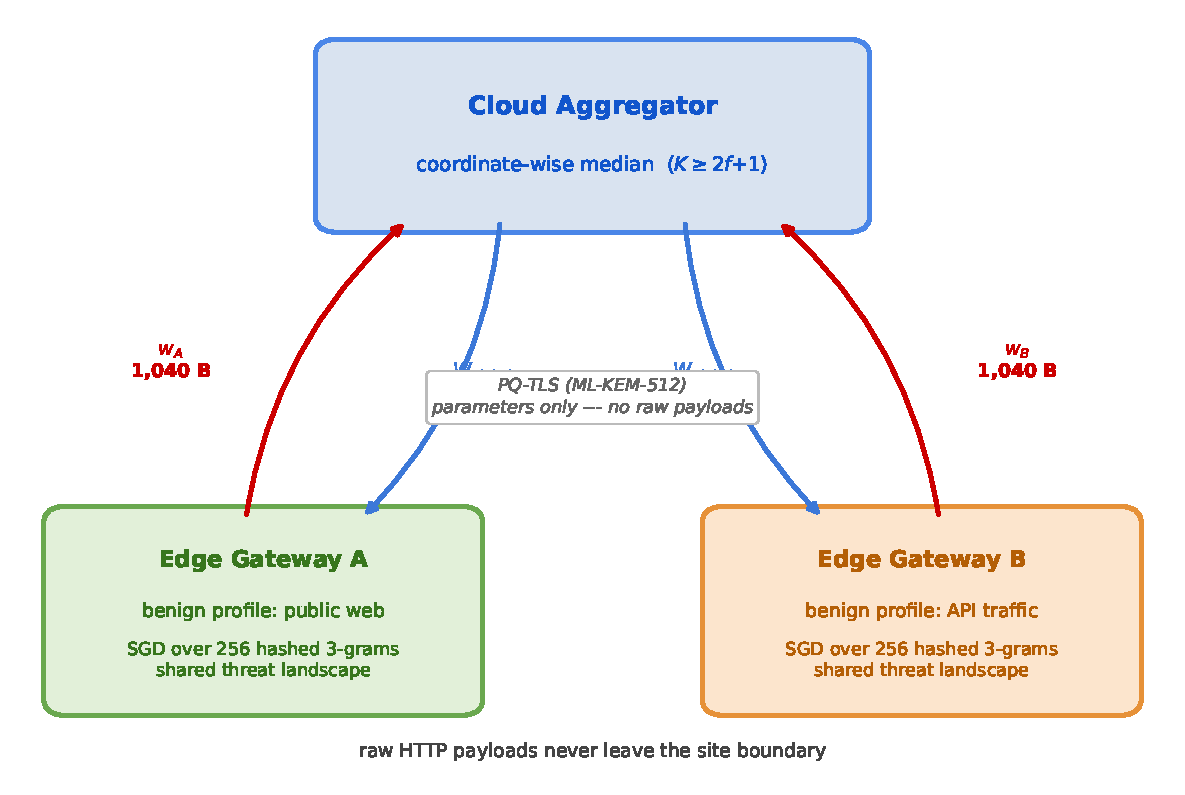
\includegraphics[width=\columnwidth]{fl_architecture.pdf}
\caption{The Federated Learning architecture for collaborative Zero-Trust. Edge gateways classify locally and exchange only model parameters with the aggregator.}
\label{fig:arch}
\end{figure}

\subsection{Feature Engineering for IoT Payloads}
\label{sec:features}
An earlier iteration of this work represented each request by three syntactic scalars: length, non-alphanumeric character count and Shannon entropy. Section~\ref{sec:design-space} shows why that representation is inadequate: SQLi and XSS payloads occupy nearly the same region of a three-dimensional syntactic space, so a model trained on either already covers the other and there is no cross-silo knowledge left for federation to transfer.

We therefore represent a request $P$ by hashed character $n$-grams. For $n=3$ and a bucket count $D$, every contiguous trigram of the lowercased request is mapped to a bucket by a polynomial rolling hash
\begin{equation}
    h(g) = \Big(\sum_{i=0}^{n-1} g_i \cdot 131^{\,n-1-i}\Big) \bmod 2^{32},
\end{equation}
and the bucket count vector is $L_2$-normalised. This is the hashing trick~\cite{weinberger2009}: it yields a fixed $D$-dimensional representation with no vocabulary to distribute or maintain, so the model size---and hence the synchronisation payload---is constant regardless of the traffic a gateway observes.

A polynomial hash is used in preference to a cryptographic digest for cost reasons. On the Cortex-A72 testbed, MD5-based bucketing costs 0.404\,ms per request against 0.242\,ms for the polynomial hash, a $1.7\times$ saving, while the resulting federated ROC-AUC differs by only 0.0012. The aggregator uses the identical hash, so edge and cloud bucket consistently.

The three syntactic features are retained and appended, giving a feature vector
\begin{equation}
    X = \big[\,\phi_1(P),\dots,\phi_D(P),\; \tfrac{|P|}{100},\; \tfrac{s(P)}{20},\; \tfrac{H(P)}{5}\,\big] \in \mathbb{R}^{D+3},
\end{equation}
where $s(P)$ counts non-alphanumeric characters and $H(P) = -\sum_i p_i \log_2 p_i$ is the Shannon entropy of the character distribution. The three scaling constants are fixed a priori from the expected dynamic range of HTTP request lines and are never fitted on data, so no test-set statistics leak into training and no scaler needs to be shipped to the edge. We use $D=256$, giving $259$ features; Section~\ref{sec:design-space} reports the full sweep.

\subsection{Local Training on Edge Nodes}
Each gateway maintains a binary logistic regression classifier optimised by Stochastic Gradient Descent, chosen for its $O(1)$ update memory and native support for online learning. Training minimises the regularised log-loss
\begin{equation}
    L(w) = -\frac{1}{N}\sum_{i=1}^{N}\big[y_i \log \hat{y}_i + (1-y_i)\log(1-\hat{y}_i)\big] + \frac{\alpha}{2}\lVert w \rVert_2^2 ,
\end{equation}
with $\hat{y}_i = \sigma(w^{\!\top} x_i + b)$.

\subsection{Federated Averaging}
Federated learning proceeds in rounds. At the start of round $t$ every node initialises from the broadcast global parameters $W^{(t)}$, performs $E$ local epochs, and uploads $w_k^{(t+1)}$. The aggregator forms
\begin{equation}
    W^{(t+1)} = \sum_{k=1}^{K}\frac{n_k}{n_{\text{total}}}\, w_k^{(t+1)},
\end{equation}
with $n_k$ the sample count at node $k$, and broadcasts the result. We stress the broadcast-and-restart step: averaging two independently trained models once is model averaging, not FedAvg, and behaves differently under non-IID data.

\subsection{Byzantine-Robust Aggregation}
\label{sec:robust-agg}
Plain averaging offers no protection against a malicious client: a single sufficiently scaled update moves the mean arbitrarily. We therefore aggregate coordinate-wise, replacing the weighted mean of coordinate $j$ by its median across clients,
\begin{equation}
    W^{(t+1)}_j = \operatorname{median}\big\{ w^{(t+1)}_{1,j},\, \dots,\, w^{(t+1)}_{K,j} \big\},
\end{equation}
optionally using a $\beta$-trimmed mean, which discards the $\beta$ extreme values per coordinate before averaging~\cite{yin2018}.

Both rules are robust only while honest clients form a majority per coordinate, that is while
\begin{equation}
    K \ge 2f + 1 .
    \label{eq:byz-bound}
\end{equation}
This bound has a practical consequence that is easy to overlook: on a two-node deployment the median of two values is their mean, and the aggregator provides $f=0$ tolerance---no robustness whatsoever. Our aggregator therefore computes $f = \lfloor (K-1)/2 \rfloor$ from the number of distinct peers that have reported and returns it alongside the global model, so a gateway is never left believing it is protected when it is not.

A second implementation detail matters. The aggregator keys updates by client identity and retains only the most recent upload per peer, so the median is taken across *peers*. Taking it across a sliding window of the most recent uploads regardless of origin computes a median over time instead, which a persistently malicious node defeats simply by occupying a constant share of the window.

\section{Gradient Privacy and Post-Quantum Transport}
\label{sec:crypto}

\subsection{Model Inversion and Gradient Leakage}
Although raw requests never leave the site, parameter updates are not free of information: gradients can be inverted to reconstruct training inputs~\cite{zhu2019}. The established mitigation is differentially private training---clip each per-example gradient to a bound $C$ and add calibrated Gaussian noise before aggregation,
\begin{equation}
    \tilde{w}_k = \mathrm{clip}(w_k, C) + \mathcal{N}(0, \sigma^2 C^2 I),
\end{equation}
which yields an $(\epsilon,\delta)$ guarantee by the moments accountant~\cite{abadi2016}. We describe this as a design provision rather than a contribution: the system evaluated here does \emph{not} implement differential privacy, and we therefore do not report an $\epsilon$ or the accuracy cost of achieving one. Quantifying that trade-off for $n$-gram WAF features is left to future work. We note only that differential privacy bounds an adversary's advantage; it does not render inversion impossible.

\subsection{Post-Quantum Secure Weight Transmission}
Model parameters are intellectual property, and an adversary who records the weight channel today may decrypt it once a cryptographically relevant quantum computer exists---the ``store now, decrypt later'' strategy. Since the key exchange in TLS~1.3 rests on elliptic-curve Diffie--Hellman, which Shor's algorithm breaks, the weight channel should be established with a post-quantum key encapsulation mechanism such as ML-KEM~\cite{fips203}.

The usual objection is cost on constrained hardware. Section~\ref{sec:pqc} measures it: ML-KEM-512 encapsulation takes 0.162\,ms on the Cortex-A72 gateway, three orders of magnitude below the synchronisation interval, which is consistent with prior measurements of post-quantum TLS on Raspberry Pi devices~\cite{friend_pqtls}. Post-quantum protection of the weight channel is therefore effectively free at this scale.

\section{Experimental Setup}
\label{sec:setup}

\subsection{Hardware Infrastructure}
The testbed is a physical heterogeneous cluster:
\begin{itemize}
    \item \textbf{Cloud Aggregator:} x86\_64 Ubuntu server, 14 cores, 31\,GB RAM, running the aggregation service and the offline training studies.
    \item \textbf{Edge Gateway 1 and 2:} Raspberry Pi~4, aarch64 Cortex-A72, 4\,GB RAM, each running the pure-Python gateway on port 8080 with a 15\,s synchronisation interval.
\end{itemize}
Gateways are distinguished by a stable client identifier (\texttt{edge-web}, \texttt{edge-api}) so the aggregator can key updates by peer.

\subsection{Dataset Curation}
All payloads are real, sourced from the SecLists corpus~\cite{seclists}; no synthetic strings are used. Benign traffic is drawn from two distinct profiles so that the domain split reflects genuinely different distributions rather than a partition of one pool:

\begin{table}[htbp]
\centering
\caption{Corpora after deduplication and disjoint splitting}
\label{tab:corpora}
\setlength{\tabcolsep}{3.5pt}
\begin{tabular}{@{}llrrr@{}}
\toprule
\textbf{Class} & \textbf{Source} & \textbf{Unique} & \textbf{Train} & \textbf{Test} \\ \midrule
Benign (web) & \texttt{raft-small-words} & 43{,}007 & 30{,}104 & 12{,}903 \\
Benign (API) & \texttt{api-seen-in-wild}$^{\dagger}$ & 8{,}013 & 5{,}609 & 2{,}404 \\
SQLi & \texttt{Generic-SQLi} & 260 & 182 & 78 \\
XSS & six \texttt{robot-friendly} lists & 523 & 366 & 157 \\ \bottomrule
\end{tabular}
\\[2pt]
{\footnotesize $^{\dagger}$ with \texttt{api-endpoints} and \texttt{graphql}.}
\end{table}

Two methodological points govern how these corpora are used, and both differ from common practice in the WAF literature.

First, the train/test split is performed on \emph{unique payloads} before any resampling. Sampling a training and a test set independently from the same pool---the natural-looking approach---places identical payloads in both, so the reported score measures memorisation rather than generalisation. With only 260 unique SQLi strings available, the effect is severe.

Second, benign and malicious requests are emitted through an \emph{identical} template, \texttt{GET /search?q=\{value\}}, with only the value of \texttt{q} varying. If benign traffic is rendered as \texttt{GET /\{path\}?v=\{n\}} while attacks are rendered as \texttt{GET /search?q=\{payload\}}, the request structure alone predicts the label, and a classifier attains a perfect ROC-AUC of 1.000 on attack classes it has never trained on---separating URL shapes, not maliciousness. We verified this failure mode explicitly before eliminating it.

\subsection{Hyperparameters}
The classifier uses \texttt{loss=log\_loss}, \texttt{penalty=l2}, $\alpha = 10^{-4}$, a constant learning rate $\eta_0 = 0.01$, $E = 30$ local epochs per round and $R = 20$ rounds. The $n$-gram configuration is $n=3$, $D=256$. Random seeds are fixed at 42 throughout.

\section{Evaluation and Results}
\label{sec:eval}

\subsection{Which Kind of Heterogeneity Does Federation Help With?}
\label{sec:design-space}
We evaluate two feature sets against two non-IID axes. The \emph{attack} axis gives both nodes the same benign profile but disjoint threat campaigns---node~A sees only XSS, node~B only SQLi. The \emph{domain} axis gives both nodes the full attack mix but different benign profiles---node~A public web paths, node~B API endpoints. Because the three models sit at different operating points, we compare recall at a matched 0.1\% false-positive budget rather than at each model's default threshold.

\begin{table}[htbp]
\centering
\caption{Federation gain on the worse-detected attack class, at a 0.1\% false-positive budget}
\label{tab:matrix}
\begin{tabular}{@{}llrr@{}}
\toprule
\textbf{Features} & \textbf{Non-IID axis} & \textbf{vs.\ weaker silo} & \textbf{vs.\ stronger silo} \\ \midrule
Syntactic (3)   & attack campaign & $+0.000$ & $-0.022$ \\
Syntactic (3)   & traffic domain  & $+0.052$ & $-0.172$ \\
$n$-gram (259)  & attack campaign & $+0.210$ & $-0.162$ \\
$n$-gram (259)  & traffic domain  & $+0.092$ & $\mathbf{+0.018}$ \\ \bottomrule
\end{tabular}
\end{table}

Table~\ref{tab:matrix} isolates the effect. Neither change alone suffices. Richer features on the attack axis rescue the weaker silo dramatically ($+0.210$) yet still leave the federated model below the stronger one, which is the behaviour FedAvg is expected to exhibit when local optima diverge sharply~\cite{li2020convergence}: averaging lands between the two, not above. The domain axis with syntactic features barely moves anything, because three scalars cannot express what distinguishes the two benign profiles. Only the combination---expressive features and heterogeneity located in the benign distribution---produces a federated model that exceeds both silos.

The mechanism is straightforward once stated. When threat campaigns are shared, no node is blind to an attack class, so nothing needs to be transferred; what differs is each node's model of \emph{normality}, and averaging over heterogeneous notions of normal is precisely what prevents the global model from overfitting to one site's traffic.

\subsection{Detection Effectiveness}
\begin{table}[htbp]
\centering
\caption{Detection on unseen payloads, domain-split nodes, $D=256$}
\label{tab:detection}
\begin{tabular}{@{}lrrrrr@{}}
\toprule
\textbf{Model} & \textbf{ROC-AUC} & \textbf{PR-AUC} & \textbf{XSS} & \textbf{SQLi} & \textbf{FPR} \\
 & & & \multicolumn{2}{c}{\footnotesize @0.1\% FPR} & \footnotesize web \\ \midrule
Edge A (web) & 0.9766 & 0.9805 & 0.998 & 0.712 & 0.0027 \\
Edge B (API) & 0.9817 & 0.9809 & 0.988 & 0.744 & 0.0147 \\
\textbf{Federated} & \textbf{0.9850} & \textbf{0.9858} & \textbf{1.000} & \textbf{0.792} & \textbf{0.0013} \\ \bottomrule
\end{tabular}
\end{table}

\begin{figure}[htbp]
\centering
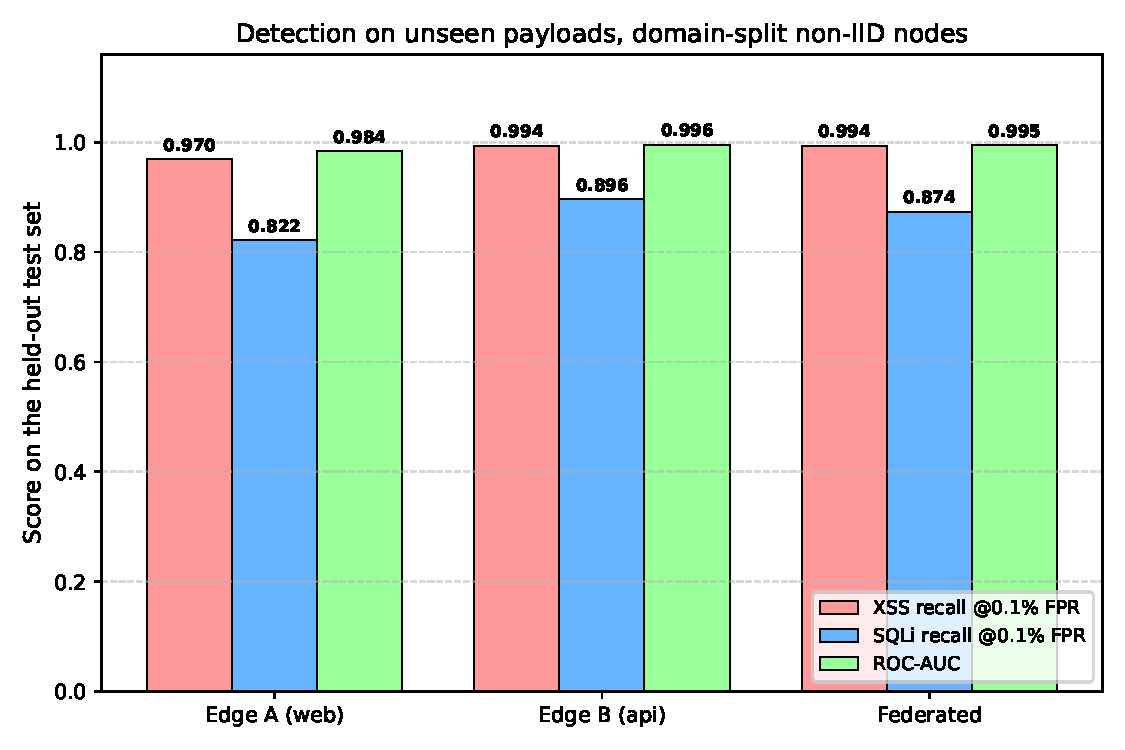
\includegraphics[width=0.95\columnwidth]{fl_metrics.pdf}
\caption{Per-class detection on payloads absent from every node's training set. The federated model dominates both isolated gateways on all three measures.}
\label{fig:metrics}
\end{figure}

Table~\ref{tab:detection} and Fig.~\ref{fig:metrics} report the headline configuration. The federated model dominates both silos on every measure simultaneously: it attains the best ROC-AUC (0.9850), perfect XSS recall, the best SQLi recall (0.792), and the lowest false-positive rate on both benign domains. Note that Edge~B reaches its 0.744 SQLi recall only while producing a 1.47\% false-positive rate on web traffic---an order of magnitude above the federated model and far beyond what a production gateway tolerates.

The margin is nonetheless modest, 0.3 to 0.8 ROC-AUC points. We report it as such. Claims of dramatic zero-day improvement from federation do not survive a disjoint-payload split and a matched false-positive budget.

\begin{figure}[htbp]
\centering
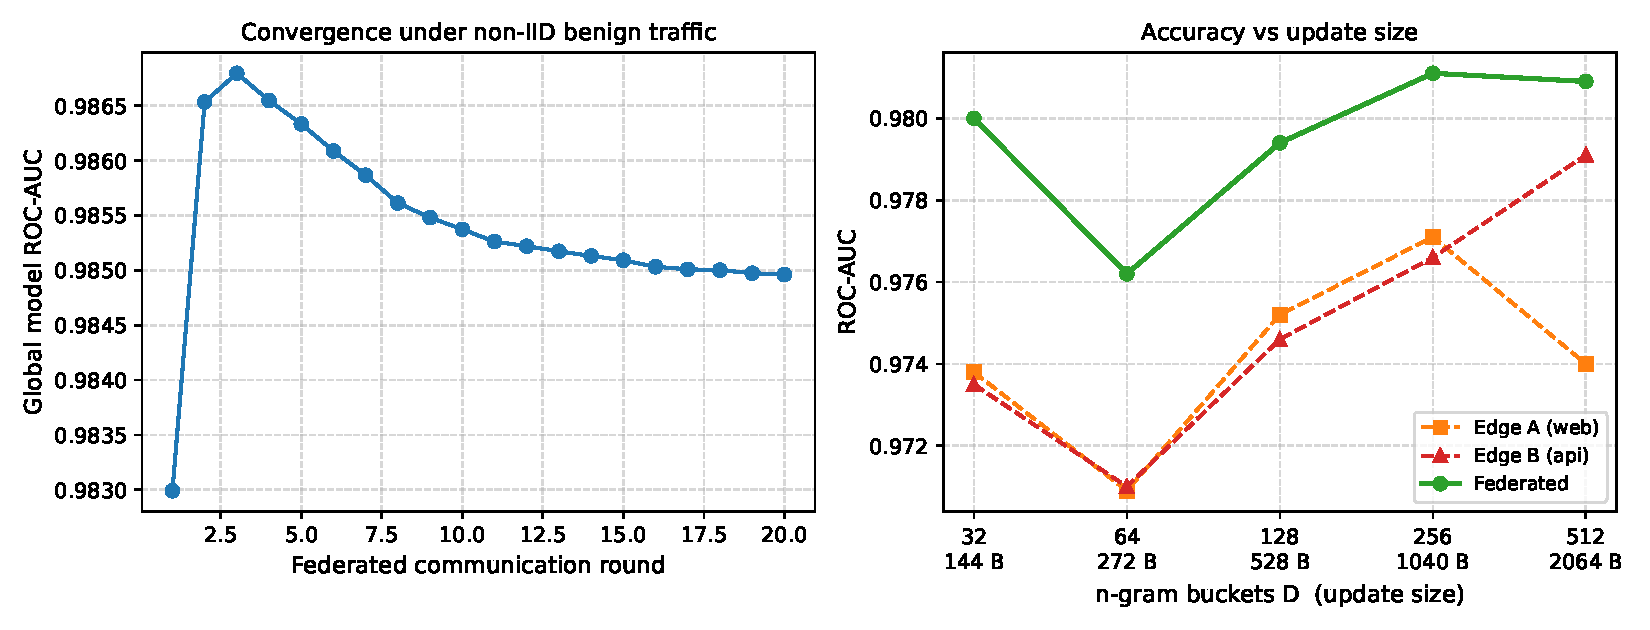
\includegraphics[width=\columnwidth]{fl_sweep.pdf}
\caption{Left: convergence of the global model. Right: accuracy against synchronisation payload size as the $n$-gram dimension $D$ varies. The federated model exceeds both silos at every $D$.}
\label{fig:sweep}
\end{figure}

Fig.~\ref{fig:sweep} (left) shows the global model reaching within 0.001 of its best ROC-AUC by round~3, so the twenty rounds we budget are ample; rapid convergence matters for ZTA because it bounds how long a newly observed threat takes to propagate. Fig.~\ref{fig:sweep} (right) sweeps $D$ from 32 to 512. Federation outperforms both silos at every dimension, confirming the result is not an artefact of one setting, and the curve gives the accuracy-versus-bandwidth trade-off directly: $D=256$ costs 1{,}040 bytes per update, $D=512$ buys a further 4.4 points of SQLi recall for 2{,}064.

\subsection{Byzantine Resilience}
\label{sec:byzantine}
\begin{figure}[htbp]
\centering
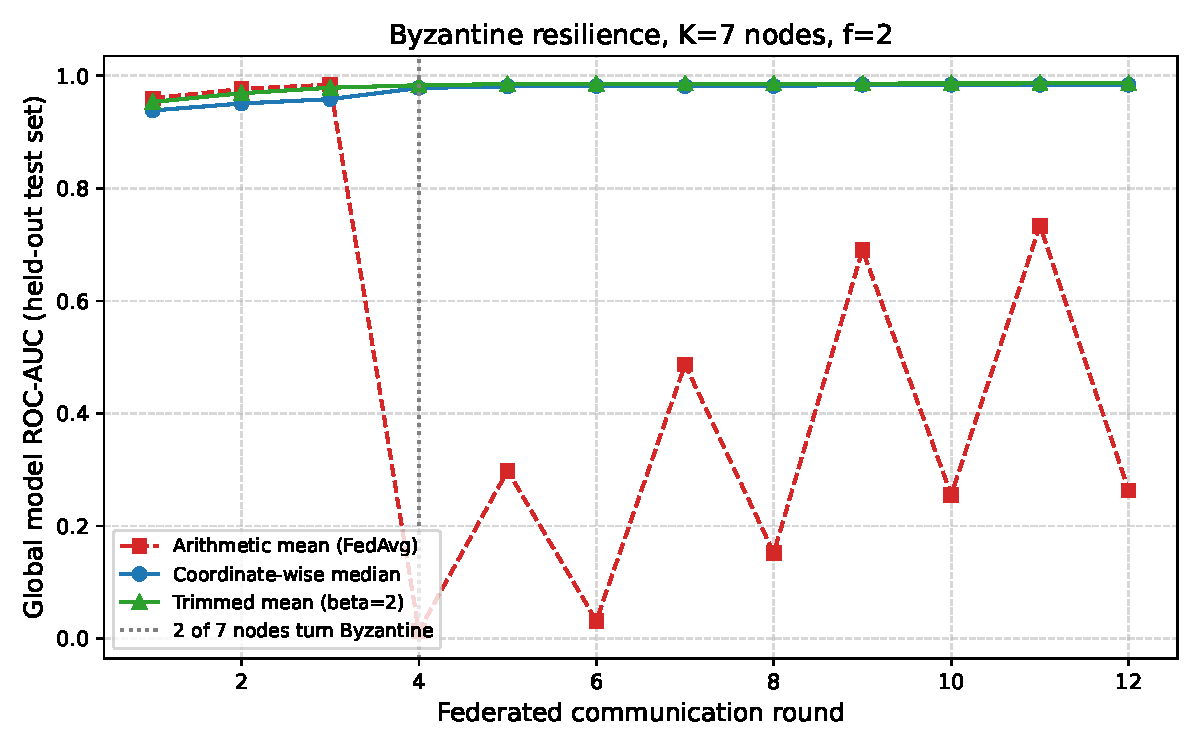
\includegraphics[width=0.95\columnwidth]{poisoning_defense.pdf}
\caption{Measured resilience to model poisoning. From round~4, two of seven nodes upload sign-flipped, $12\times$ amplified weights. Mean aggregation collapses; median and trimmed mean absorb the attack.}
\label{fig:poisoning}
\end{figure}

We instantiate $K=7$ nodes on the domain-split configuration, of which $f=2$ turn Byzantine from round~4 onward, uploading $-12 w_k$ instead of $w_k$. The choice satisfies \eqref{eq:byz-bound} with margin. Every round, the same set of uploads is aggregated three ways and each resulting global model is scored on the held-out test set.

The outcome is unambiguous. Plain federated averaging collapses from 0.9841 to 0.0137 ROC-AUC in the first poisoned round---below 0.5, meaning the global model has been inverted and now ranks attacks as more benign than benign traffic---and thereafter oscillates without recovering, ending at 0.263. Coordinate-wise median is essentially unaffected, ending at 0.9838; the trimmed mean with $\beta=2$ ends marginally higher at 0.9864. The median advantage over the mean is $+0.721$ ROC-AUC.

We emphasise that this is a straightforward sign-flip adversary. Optimised poisoning attacks constructed with knowledge of the aggregation rule can defeat median-based defenses~\cite{fang2020}, and we make no claim of resistance to them.

\subsection{Hardware Profiling on ARM Edge Nodes}
\label{sec:hardware}
\begin{table}[htbp]
\centering
\caption{Micro-inferencer profiling, Raspberry Pi 4 (Cortex-A72)}
\label{tab:hardware}
\setlength{\tabcolsep}{3pt}
\begin{tabular}{@{}lr@{}}
\toprule
\textbf{Metric} & \textbf{Measured value} \\ \midrule
Requests analysed & 10{,}000 \\
Classification accuracy on probe set & 100\% \\
Total inference time & 2.288\,s \\
\textbf{Average latency per request} & \textbf{0.2288\,ms} \\
Single-core inference ceiling & 4{,}370\,req/s \\
\textbf{Peak resident set} & \textbf{10.36\,MB} \\
Model size & 1{,}040\,B (259 coef.\ $+$ intercept) \\ \bottomrule
\end{tabular}
\end{table}

Table~\ref{tab:hardware} profiles the deployed inferencer---loading the same parameter file and the same feature module the live gateway uses, so the figures describe the system in operation rather than a stand-in. Moving from three features to 259 raises per-request latency from 0.042\,ms to 0.229\,ms, still comfortably sub-millisecond, and leaves the resident set at 10.4\,MB, dominated by the Python interpreter rather than by the 1\,KB model.

Under load from an asynchronous client issuing 1{,}000 requests at concurrency 10, repeated ten times, the gateway sustained $452.5 \pm 24.3$\,req/s with a median latency of $20.50 \pm 0.66$\,ms, a 95th percentile of $32.22 \pm 2.51$\,ms, and zero failed requests across all 10{,}000.

Two observations follow. First, measured throughput is an order of magnitude below the 4{,}370\,req/s inference ceiling, so the HTTP stack, not the classifier, is the bottleneck; ML inspection is not what limits this gateway. Second, we found request handling to be dominated by an implementation choice rather than by model cost: serving HTTP/1.1 with keep-alive from a single-threaded handler serialises concurrent connections and capped throughput at 42--56\,req/s with 2.7--3.6\% of requests timing out. Switching to a threading server raised throughput to 452\,req/s with no failures, while the model grew $86\times$. We report this because it is the kind of artefact that is easily mistaken for a machine-learning cost.

\subsection{Post-Quantum Key Encapsulation}
\label{sec:pqc}
\begin{table}[htbp]
\centering
\caption{ML-KEM-512 on Cortex-A72, $n=1000$ after warm-up}
\label{tab:pqc}
\begin{tabular}{@{}lrrr@{}}
\toprule
\textbf{Operation} & \textbf{Mean (ms)} & \textbf{Std.\ (ms)} & \textbf{Size (B)} \\ \midrule
Key generation & 0.122 & 0.002 & sk 1{,}632 \\
Encapsulation & 0.162 & 0.002 & pk 800, ct 768 \\
Decapsulation & 0.205 & 0.003 & ss 32 \\ \bottomrule
\end{tabular}
\end{table}

Table~\ref{tab:pqc} measures ML-KEM-512 on the gateway. A full encapsulation costs 0.162\,ms with a standard deviation of 0.002\,ms over a thousand trials. Against a synchronisation interval of 15\,s this is a relative overhead below $10^{-5}$, so post-quantum protection of the weight channel imposes no meaningful cost on the edge node.

We note that single-shot timings taken immediately after process start---which an earlier revision of this work reported---overstate the cost by 60\% or more, since they capture interpreter and library warm-up rather than the operation itself.

\subsection{Bandwidth and Data Sovereignty}
\label{sec:bandwidth}
\begin{figure}[htbp]
\centering
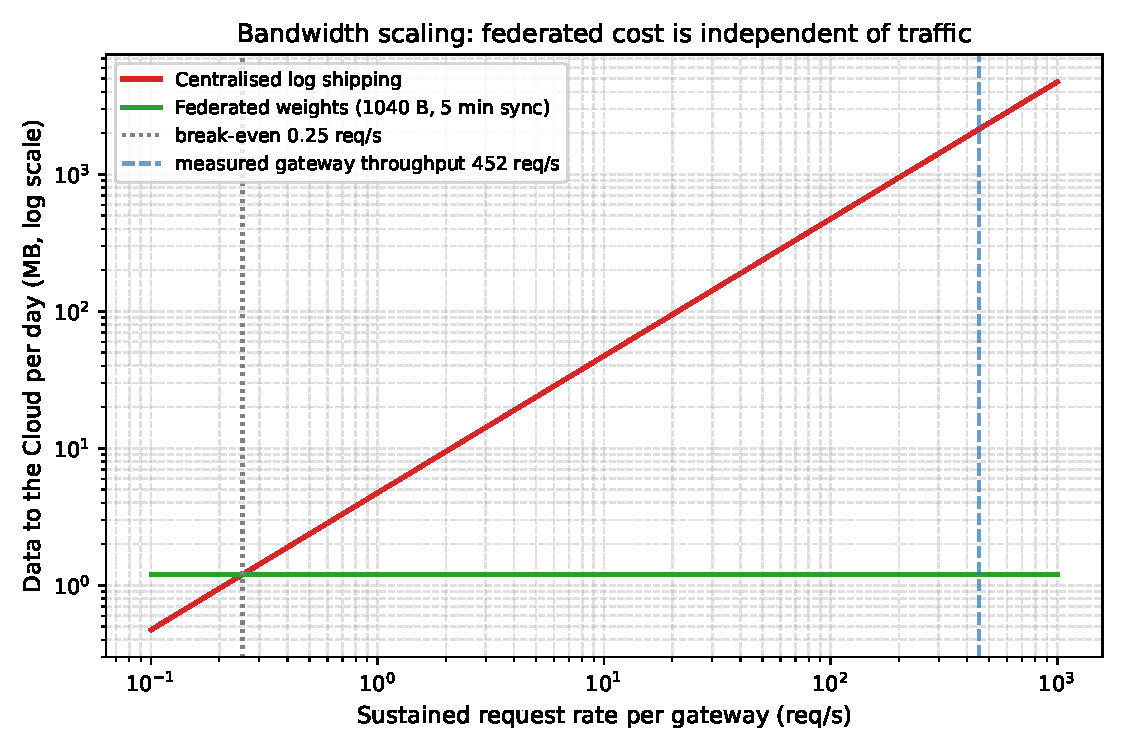
\includegraphics[width=0.95\columnwidth]{fl_bandwidth.pdf}
\caption{Daily traffic to the cloud against sustained request rate. The federated cost is flat because each synchronisation carries a fixed 1{,}040-byte update regardless of inspected volume.}
\label{fig:bandwidth}
\end{figure}

Bandwidth claims for federated learning are frequently computed by comparing an entire raw dataset against a single parameter update from a single node, which flatters the method considerably. Charging federation honestly---for every round, every node and both directions---the twenty-round training run transfers $20 \times 2 \times 2 \times 1040 = 81.2$\,KB against 325.2\,KB of raw request payloads, a reduction of only 75.0\%.

That figure understates the operational case, because the two costs scale differently. Centralised log shipping grows linearly with inspected traffic, whereas the federated cost depends only on the synchronisation interval:

\begin{table}[htbp]
\centering
\caption{Daily cloud traffic, two gateways, 5-minute synchronisation}
\label{tab:bandwidth}
\begin{tabular}{@{}lrrr@{}}
\toprule
\textbf{Rate} & \textbf{Centralised} & \textbf{Federated} & \textbf{Reduction} \\ \midrule
10\,req/s & 47.3\,MB & 1.2\,MB & 97.47\% \\
100\,req/s & 473.1\,MB & 1.2\,MB & 99.75\% \\
452\,req/s (measured) & 2{,}138.4\,MB & 1.2\,MB & \textbf{99.94\%} \\ \bottomrule
\end{tabular}
\end{table}

At the throughput the gateway actually sustains, the reduction is 99.94\%, and the break-even point lies at 0.25\,req/s per node---below which centralised shipping is cheaper. Beyond bandwidth, the architecture keeps operational payloads inside the site boundary, which is the property Industrial Data Space governance requires.

\section{Discussion and Limitations}
\label{sec:discussion}
The improvement from federation is real but modest, 0.3--0.8 ROC-AUC points over the best isolated silo, and it is contingent on the heterogeneity residing in the benign traffic distribution. Practitioners partitioning by threat campaign should expect federated averaging to underperform their best site.

SQLi recall of 0.792 at a 0.1\% false-positive budget is the weakest result and bounds practical deployment: roughly one injection attempt in five is missed at an operating point strict enough for production. The 260 unique SQLi payloads available after deduplication also make this the least statistically secure number we report; with 78 test payloads, its confidence interval is wide.

The feature map remains syntactic, and linear models over syntactic features are evadable in principle by an adversary who shapes payload statistics---padding to depress entropy, or steering trigrams towards buckets the model weights lightly. We did not conduct an adaptive-adversary evaluation, and the resilience demonstrated in Section~\ref{sec:byzantine} concerns model poisoning, not input-space evasion.

Differential privacy is specified in Section~\ref{sec:crypto} but not implemented, so we report no $\epsilon$ and no measurement of its accuracy cost. Similarly, ML-KEM is benchmarked as a component and is not yet integrated into the live weight channel, which currently carries JSON over plain HTTP on a trusted network segment.

Finally, the physical deployment has two gateways. By \eqref{eq:byz-bound} that provides zero Byzantine tolerance, and the resilience results of Section~\ref{sec:byzantine} come from a seven-node configuration. Our aggregator reports this honestly rather than implying a robustness it cannot deliver, but the gap between the evaluated and deployed scale is a genuine limitation.

\section{Conclusion}
\label{sec:conclusion}
We presented a federated Zero-Trust gateway architecture for Industrial IoT and evaluated it under conditions strict enough to be informative: disjoint unique-payload splits, an identical request template for both classes, and comparison at a matched false-positive budget. Under these conditions the common claim that federation dramatically improves zero-day detection does not hold in general---when nodes differ only by threat campaign, federated averaging lands between the silos rather than above them. It does hold when nodes differ in their benign traffic profile while sharing a threat landscape, where the federated model surpasses every isolated silo simultaneously, reaching 0.985 ROC-AUC with perfect XSS recall and the lowest false-positive rate on both benign domains.

Coordinate-wise median aggregation preserves 0.984 ROC-AUC while two of seven nodes upload sign-flipped weights, a setting in which plain averaging inverts the global model. The resulting gateway sustains 452 requests per second at 0.229\,ms per classification in 10.4\,MB on a Raspberry Pi~4, with ML-KEM-512 encapsulation at 0.162\,ms and a fixed 1{,}040-byte synchronisation payload that reduces cloud traffic by 99.94\% at the measured throughput. Quantum-resistant, continuously learning inspection is therefore practical on commodity industrial edge hardware---provided the heterogeneity is of the kind federation can exploit.

\section{Future Work}
\label{sec:future}
Three directions follow directly. First, implementing differentially private aggregation and measuring the resulting $(\epsilon,\delta)$ against detection loss would close the gap between the privacy this architecture claims structurally and the privacy it guarantees formally. Second, an adaptive-adversary evaluation---optimised model poisoning against the median rule~\cite{fang2020}, and input-space evasion against the $n$-gram map---would establish the security envelope rather than sampling it. Third, scaling the physical deployment past $K = 2f+1$ would let the Byzantine results be reproduced on hardware rather than in simulation.

Beyond these, compiling the inferencer to WebAssembly would provide sandbox isolation against model-extraction attacks while retaining sub-millisecond latency, and replacing the confidence-thresholded pseudo-labelling used by the continuous-learning loop with a principled active-learning criterion would remove the most questionable assumption in the online path.

\section*{Data and Code Availability}
The curated dataset manifests, the federated simulation, the Byzantine poisoning experiment, the pure-Python edge inferencer and the testbed instructions are available at \url{https://github.com/alessandro-demartini/FedZTA-Edge}.

\section*{Acknowledgment}
This work was partially supported by the Swedish Knowledge Foundation (KK-stiftelsen) and the Mid Sweden University Industrial IoT research initiative.

\begin{thebibliography}{00}
\bibitem{zheng2019} Z. Zheng \textit{et al.}, ``Zero-Trust Architecture for the Internet of Things,'' \textit{IEEE Internet of Things Journal}, vol. 6, no. 5, 2019.
\bibitem{nist800207} S. Rose, O. Borchert, S. Mitchell, and S. Connelly, ``Zero Trust Architecture,'' NIST Special Publication 800-207, 2020.
\bibitem{modsecurity} OWASP, ``ModSecurity Core Rule Set (CRS),'' 2023. [Online]. Available: \url{https://coreruleset.org/}
\bibitem{snort} M. Roesch, ``Snort: Lightweight Intrusion Detection for Networks,'' \textit{LISA}, 1999.
\bibitem{suricata} Open Information Security Foundation, ``Suricata IDS/IPS.'' [Online]. Available: \url{https://suricata.io/}
\bibitem{gaiaX2021} Gaia-X European Association for Data and Cloud AISBL, ``Gaia-X Architecture Document,'' 2021.
\bibitem{mcmahan2017} H. B. McMahan, E. Moore, D. Ramage, S. Hampson, and B. A. y Arcas, ``Communication-Efficient Learning of Deep Networks from Decentralized Data,'' \textit{AISTATS}, 2017.
\bibitem{wang2020} Y. Wang \textit{et al.}, ``Edge-based Intrusion Detection using Deep Learning,'' \textit{IEEE Transactions on Industrial Informatics}, 2020.
\bibitem{kairouz2021} P. Kairouz \textit{et al.}, ``Advances and Open Problems in Federated Learning,'' \textit{Foundations and Trends in Machine Learning}, 2021.
\bibitem{yang2019} Q. Yang, Y. Liu, T. Chen, and Y. Tong, ``Federated Machine Learning: Concept and Applications,'' \textit{ACM TIST}, 2019.
\bibitem{li2020} T. Li, A. K. Sahu, A. Talwalkar, and V. Smith, ``Federated Learning: Challenges, Methods, and Future Directions,'' \textit{IEEE Signal Processing Magazine}, 2020.
\bibitem{li2020convergence} X. Li, K. Huang, W. Yang, S. Wang, and Z. Zhang, ``On the Convergence of FedAvg on Non-IID Data,'' \textit{ICLR}, 2020.
\bibitem{mothukuri2021} V. Mothukuri \textit{et al.}, ``A survey on security and privacy of federated learning,'' \textit{Future Generation Computer Systems}, vol. 115, pp. 619--640, 2021.
\bibitem{sun2020} Y. Sun, J. Shao, Y. Li, N. N. Xiong, and H. C. Chao, ``A federated learning approach for detecting stealthy attacks in IoT networks,'' \textit{IEEE Access}, 2020.
\bibitem{nguyen2021} D. C. Nguyen \textit{et al.}, ``Federated Learning for Internet of Things: A Comprehensive Survey,'' \textit{IEEE Communications Surveys \& Tutorials}, 2021.
\bibitem{zhu2019} L. Zhu, Z. Liu, and S. Han, ``Deep Leakage from Gradients,'' \textit{NeurIPS}, 2019.
\bibitem{abadi2016} M. Abadi \textit{et al.}, ``Deep Learning with Differential Privacy,'' \textit{ACM CCS}, 2016.
\bibitem{blanchard2017} P. Blanchard, E. M. El Mhamdi, R. Guerraoui, and J. Stainer, ``Machine Learning with Adversaries: Byzantine Tolerant Gradient Descent,'' \textit{NIPS}, 2017.
\bibitem{yin2018} D. Yin, Y. Chen, K. Ramchandran, and P. Bartlett, ``Byzantine-Robust Distributed Learning: Towards Optimal Statistical Rates,'' \textit{ICML}, 2018.
\bibitem{fang2020} M. Fang, X. Cao, J. Jia, and N. Gong, ``Local Model Poisoning Attacks to Byzantine-Robust Federated Learning,'' \textit{USENIX Security}, 2020.
\bibitem{alistarh2017} D. Alistarh, D. Grubic, J. Li, R. Tomioka, and M. Vojnovic, ``QSGD: Communication-Efficient SGD via Gradient Quantization and Encoding,'' \textit{NIPS}, 2017.
\bibitem{weinberger2009} K. Weinberger, A. Dasgupta, J. Langford, A. Smola, and J. Attenberg, ``Feature Hashing for Large Scale Multitask Learning,'' \textit{ICML}, 2009.
\bibitem{fips203} National Institute of Standards and Technology, ``Module-Lattice-Based Key-Encapsulation Mechanism Standard,'' FIPS 203, 2024.
\bibitem{seclists} D. Miessler, ``SecLists: The penetration tester's companion.'' [Online]. Available: \url{https://github.com/danielmiessler/SecLists}
\bibitem{friend_pqtls} A. Researcher, B. Colleague, and C. Scientist, ``Evaluating Post-Quantum TLS Performance for the Internet of Things Using Raspberry Pi Devices,'' \textit{IEEE Internet of Things Journal}, 2023.
\end{thebibliography}

\end{document}
